\newpage

\chapter{Описание методов моделирования систем}
\section{Введение}

    В современном мире средства вычислительной техники широко используются во многих отраслях деятельности человека. Основной их задачей является обработка и хранение информации поступающей из вне. Такие системы должны обеспечивать доступ к данным и гарантировать их актуальность. Для решения проблемы быстрого получения информации конечным пользователям, отдельные компьютеры объединяются в локальные сети. Подобное объединение можно проследить вплоть до глобальной сети интернет. Однако, решив проблему, связанную с доступностью информации, соединение компьютеров обострило проблемы связанные с безопасностью данных. В случае с локальной машиной не имеющей активного сетевого соединения проблема безопасности решается ограничение физического доступа к терминалу, однако объединив рабочие станции, зона, которую необходимо контролировать, резко возрастает. Кроме того, с внедрением беспроводных технологий, это зона не имеет четких границ, а существующее подключение сети к интернет открывает потенциальную возможность для атаки человеку из любой точки мира. В зависимости от сложности архитектуры, от используемого оборудования и уровня подготовленности сотрудников, имеющих подключение к локальной сети, обнаружение и ликвидация уязвимостей резко возрастает. Принимая во внимание вышеперечисленные факторы, инженеру, ответственному за построение локальной сети, необходимо иметь возможность оценки того или иного архитектурного или программного решения с точки зрения актуальности его применения для конкретной ситуации. Для подобного рода оценок существуют различные методы и средства моделирования.

    Применение методов моделирования на этапе проектирования сети позволяет предугадать возможные проблемы при реализации выбранного решения, а также принять меры по обеспечению безопасного функционирования системы. К таким мерам относятся аппаратные средства, ограничивающие доступ к защищаемым ресурсам, протоколы криптографической защиты, программное обеспечение с возможностью мониторинга состояния сети. Различные источники придерживаются разных определений процесса моделирования, так как крайне сложно подобрать такое определение, которое в полной мере охватило деятельность по моделированию. Определение модели по А. А. Ляпунову: Моделирование – это опосредованное практическое или теоретическое исследование объекта, при котором непосредственно изучается не сам интересующий нас объект, а некоторая вспомогательная искусственная или естественная система (модель):

    \begin{itemize}
        \item находящаяся в некотором объективном соответствии с познаваемым объектом;
        \item способная замещать его в определенных отношениях;
        \item дающая при её исследовании, в конечном счете, информацию о самом моделируемом объекте;
    \end{itemize}

    "Модель (лат. modulus – мера) – это объект заместитель объекта-оригинала, обеспечивающий изучение некоторых свойств оригинала. Замещение одного объекта другим с целью получения информации о важнейших свойствах объекта-оригинала с помощью объекта-модели называется моделированием.Под математическим моделированием будем понимать процесс установления соответствия данному реальному объекту некоторого математического объекта, называемого математической моделью, иисследование этой модели, позволяющее получать характеристики рассматриваемого реального объекта. Вид математической модели зависит как от природы реального объекта, так и задач исследования объекта и требуемой достоверности и точности решения этой задачи."[1] Основная сложность математического моделирования заключается в том, что исследуемые процессы необходимо формализовать математическими функциями, что не всегда возможно. Некоторые процессы, например, действия пользователя в системе, сложно свести к математическим функциям.

    Имитационное моделирование – это метод, позволяющий строить модели, описывающие процессы так, как они проходили бы в действительности. Отличительными чертами данного метода является то, что у исследователя есть возможность изменять параметры системы, изучать процесс с одними входными данными или некоторым набором, исследовать развитие процесса во времени. Имитационное моделирование применяется тогда, когда неэффективно с точки зрения затраченных ресурсов и полученных результатов экспериментировать на реальном объекте. Невозможно построить математическую модель в связи с присутствующими в системе нелинейностях, стохастическими переменными или если необходимо исследовать систему во времени. Существующие программные решения позволяют строить модели компьютерных сетей, и исследовать с помощью этой модели различные процессы, происходящие в системе. Однако большинство таких решений созданы для использования системными администраторами, и поэтому позволяют исследовать характеристики системы безотносительно к безопасности. Данные, полученные при использовании такой системы, могут быть абсолютно бесполезными для инженера по безопасности. Существующие решения, отражающие работу сети с точки зрения безопасности являются коммерческими, что затрудняет их использование в образовательных целях или являются свободно распространяемыми, но в этом случае, обычно, обладают малым числом возможностей и неудобным для использования графическим интерфейсом. Таким образом целью данной работы является создание стенда для моделирования работы вычислительной сети с точки зрения информационной безопасности. Данный стенд должен предоставлять возможность построения сетей различных архитектур и топологий, выявлять "узкие"места в локальной сети замедляющие ее работу или представляющие собой уязвимость, а так же изучить состояние и поведение системы при различного рода атаках. В качестве объекта исследования будем рассматривать процесс моделирования взаимодействия различных устройств, объединенных в вычислительную сеть. В рамках данной работы будет построена система, позволяющая моделировать алгоритмы работы устройств на различных уровнях эталонной модели взаимодействия открытых систем(OSI). Протоколы транспортного сетевого и канального уровней возможно моделировать без привлечения математических моделей и аппарата математической статистики. В то время как более высокие уровни взаимодействия связаны с действиями пользователя в системе и не могут быть точно воспроизведены. В связи с этим при моделировании генерации трафика в сети, то есть обычного режима работы, будут использованы математические модели, построенные при исследовании данного явления. При моделировании работы протоколов нижнего уровня и физической передачи данных возникаю проблемы иного характера. Они связаны в первую очередь с наличием ошибки в канале связи. Учитывая то, что в реальных условиях эта ошибка носит, преимущественно, случайный характер, моделирование подобных инцидентов будет проводится с использованием методов математической статистки.

    Для построения модели вычислительной сети будет применен метод имитационного моделирования. Благодаря этому методу система будет иметь необходимую гибкость при настройке параметров. Наиболее удобным видом моделирования для данной задачи является метод агентного моделирования, так как он позволяет описывать поведение каждого компонента системы в отдельности, а так же порядок их взаимодействия. Описанные преимущества позволяют произвести декомпозицию задачи и построить систему необходимого уровня сложности.

    Для построения целевой системы необходимо разработать архитектуру будущего приложения. Она должна включать в себя возможности по построению моделей вычислительных сетей различной конфигурации, предусматривать механизмы настройки большинства компонентов системы, обладать гибкостью для возможного расширения используемого оборудования и протоколов. Следующим этапом разработки является алгоритмизация математических моделей, описывающих генерацию трафика пользователем в вычислительной сети. Результатом данного этапа будет система, в достаточной степени точно отражающая реальные процессы, протекающие в вычислительной сети. Третьим этапом разработки станет подсистема сбора статистической информации по различным устройствам. Данная подсистема занимается сбором данных со всех устройств, входящих в состав моделируемой сети и позволяет проследить динамику изменения состояний различных узлов. Заключительным этапом является создание подсистемы, моделирующей различные виды атак на локальную сеть. В рамках данной подсистемы описываются устройства и программы(алгоритмы), используемые при атаках на вычислительные сети, определяются механизмы подключение к локальной сети, моделируются действия злоумышленника. По последнему пункту будет рассмотрено такое понятие, как мотивация злоумышленника, которая влияет на его заинтересованность в компрометации системы.

    Для решения поставленных задач будет использоваться язык программирования JAVA с использованием различных расширений.




\section{Классификация видов моделирования.}

\subsection{Классификационные признаки.}

 В качестве одного из первых признаков классификации видов моделирования можно выбрать степень полноты модели и разделить модели в соответствии с этим на полные, неполные и приближенные. В основе полного моделирования лежит полное подобие, которо проявляется как во времени, так и в пространстве. Для неполного моделирования характерно неполное подобие модели изучаемому объекту. В основе приближенного моделирования лежит приближенное подобие, при котором некоторые стороны функционирования реального объекта не моделируются совсем.

    В зависимости от характера изучаемых процессов в системе S все виды моделирования могут быть разделены на детерминированные и стохастические, статические и динамические, дискретные, непрерывные и дискретно-непрерывные. Детерминированное моделирование отображает детерминированные процессы, т.е. процессы, в которых предполагается отсутствие всяких случайных воздействий; стохастическое моделирования отображает вероятностные процессы и события. В этом случае анализируется ряд реализаций случайного процесса и оцениваются средние характеристики, т.е. набор однородных реализаций. Статическое моделирования служит для описания поведения объекта в какой-либо момент времени, ф динамическое моделирование отражает поведение объекта во времени. Дискретное моделирование служит для описания процессов, которые предполагаются дискретными, соответственно непрерывное моделирование используется для случаев, когда хотят выделить наличие как дискретных, так и непрерывных процессов.[1]


\subsection{Математическое моделирование.}

 Для исследования характеристик процесса функционирования любой системы S математическими методами, включая и машинные, должна быть проведена формализация этого процесса, т.е. построена математическая модель.

    Под математическим моделированием понимают процесс установления соответствия данному реальному объекту некоторого математического объекта, называемого математической моделью, и исследование этой модели, позволяющее получать характеристики рассматриваемого реального объекта. Вид математического модели зависит как от природы реального объекта, так и задач исследования объекта и требуемой достоверности и точности решения этой задачи. Любая математическая модель, как и всякая другая описывает реальный объект лишь с некоторой степенью прближения к действительности. Математическое моделирование для исследвания характеристик процесса функционирования систем можно разделить на аналитическое, имитационное и комбинированное.

    Для аналитического моделирования характерно то, что процессы функционирования элементов системы записываются в виде некоторых функциональных соотношений (алгебраических, интегродифференциальных, конечно-разностных и.т.п.) или логических условий. Аналитическая модель может быть исследована следующими методами:
\begin{enumerate}
  \item аналитическим, когда стремятся получить в общем виде явные зависимости для искомых характеристик;
  \item численным, когда, не умея решать уравнений в общем виде, стремятся получить числовые результаты при конкретных начальных данных;
  \item качественным, когда, не имея решения в явном виде, можно найти некоторые свойства решения.
\end{enumerate}

    Наиболее полное исследование процесса функционирования системы можно провести, если известны явные зависимости, связывающие искомые характеристики с начальными условиями, параметрами и переменными системы S. Однако такие зависимости удается получить только для сравнительно простых систем. При усложнении систем исследование их аналитическим методом наталкивается на значительные трудности, которые часто бывают непреодолимыми. Поэтому, желая использовать аналитический метод, в этом случае идут на существенное упрощение первоначальной модели, чтобы иметь возможность изучить хотя бы общие свойства системы. Такое исследование на упрощенной модели аналитическим методом помогает получить ориентировочные результаты для определения более точных оценок другими методами. Численный метод позволяет исследовать по сравнению с аналитическим методом более широкий класс систем, но при этом полученные решения носят частный характер. Численный метод особенно эффективен при использовании ЭВМ.

    В отдельных случаях исследования системы могут удовлетворять и те выводы, которые можно сделать про использовании качественного метода анализа математической модели. Такие качественные методы широко используются, например, в теории автоматического управления для оценки эффективности различных вариантов систем управления.

    В настоящее время распространены методы машинной реализации исследования характеристик процесс функционирования больших систем. Для реализации математической модели на ЭВМ необходимо построить соответствующий моделирующий алгоритм.

    При имитационном моделировании реализующий модель алгоритм воспроизводит процесс функционирования системы S во времени, причем имитируются элементарные явления, составляющие процесс, с сохранением их логической структуры и последовательности протекания во времени , что позволяет по исходным данным получить сведения о состояниях процесса в определенные моменты времени, дающие возможность оценить характеристики системы S.

    Основным преимуществом имитационного моделирования по сравнению с аналитическим является возможность решения более сложных задач. Имитационные модели позволяют достаточно просто учитывать такие факторы, как наличие дискретных и непрерывных элементов, нелинейные характеристики элементов системы, многочисленные случайные воздействия и др., котоые часто создают трудности при аналитических исследованиях. В настоящее время имитационное моделирование -- наиболее эффективный метод исследования больших систем, а часто и единственный практически доступный метод получения информации о поведении системы, особенно на этапе ее проектирования.
    Когда результаты, полученные про воспроизведении на имитационной модели процесса функционирования системы S, являются реализациями случайных величин и функций, тогда для нахождения характеристик процесса требуется его многократное воспроизведение с последующей статистической обработкой информации и целесообразно в качестве метода машинной реализации имитационной модели использовать метод статистического моделирования. Первоначально был разработан метод статистических испытаний, представляющий собой численный метод, который применялся для моделирования случайных величин и функций, вероятностные характеристики которых совпадали с решениями аналитических задач (такая процедура получила название метода Монте-Карло). Затем этот прием стали применять и для машинной имитации с целью исследования характеристик процессов функционирования систем, подверженных случайным воздействиям, т.е. появился метод статистического моделирования. Таким образом, методом статистического моделирования называют метод машинной реализации имитационной модели, а методом статистических испытаний -- численный метод решения аналитической задачи.

    Метод имитационного моделирования позволяет решать задачи анализа больших систем, включая задачи оценки: вариантов структуры систем, эффективности различных алгоритмов управления системой, влияния изменения различных параметров системы. Имитационное моделирование может быть положено также в основу структурного. алгоритмического и параметрического синтеза больших систем, когда требуется создать систему, с заданными характеристиками при определенных ограничениях, которая является оптимальной по некоторым критериям оценки эффективности.

    При решении задач машинного синтеза систем на основе их имитационных моделей помимо разработки моделирующих алгоритмов для анализа фиксированной системы необходимо так же разработать алгоритмы поиска оптимального варианта системы. Далее в методологии машинного моделирования будем различать два основных раздела: статику и динамику, -- основным содержанием которых являются соответственно вопросы анализа и синтеза систем, заданных моделирующими алгоритмами.

    Комбинированное (аналитико-имитационное) моделирование при анализе и синтезе систем позволяет объединить достоинства аналитического и имитационного моделирования. При построении комбинированных моделей проводится предварительная декомпозиция процесса функционирования объекта на составляющие подпроцессы и для тех из них, где это возможно, используются аналитические модели, а для остальных подпроцессов строятся имитационные модели. Такой комбинированный подход позволяет охватить качественно новые классы систем, которые не могут быть исследованы с использованием только аналитического и имитационного моделирования в отдельности.[1]


\subsubsection{Формальная модель объекта.}

Модель объекта моделирования, т. е. системы S, можно представить в виде множества величин, описывающих процесс функционирования реальной системы и образующих в общем случае следующие подмножества:

\begin{enumerate}
  \item совокупность входных воздействий на систему
      \begin{center}
        $x_{i} \in X, i = \sup{1, n_{X}}$; х,еХ, i=l , пх;
      \end{center}

  \item совокупность воздействий внешней среды
     \begin{center}
       $\upsilon_{l} \in V l = \sup{1, n_{V}}$;
     \end{center}

  \item совокупность внутренних (собственных) параметров системы
     \begin{center}
       $h_{k} \in H, k = \sup{1, n_{H}}$;
     \end{center}

  \item совокупность выходных характеристик системы
    \begin{center}
      $y_{j} \in Y, j = \sup{1, n_{Y}}$
    \end{center}

\end{enumerate}

  При этом в перечисленных подмножествах можно выделить управляемые и неуправляемые переменные. В общем случае $x_{i}$, $\upsilon_{l}$, $h_{k}$, $y_{j}$ являются элементами непересекающихся подмножеств и содержат как детерминированные, так и стохастические составляющие. При моделировании системы S входные воздействия, воздействия внешней среды Е и внутренние параметры системы являются независимыми (экзогенными) переменными, которые в векторной форме имеют соответственно вид $\vec{x}(t) = (x_{1}(t), x_{2}(t), ..., x_{nX}(t))$; $\vec{v}(t) = (v_{1}(t), v_{2}(t), ... , v_{nV}(t))$; $\vec{h}(t) = (h_{1}(t), h_{2}(t), ... , h_{nH}(t))$, а выходные характеристики системы являются зависимыми (эндогенными) переменными и в векторной форме имеют вид $\vec{y}(t) = (y_{1}(t), y_{2}(t), ... , y_{nY}(t))$.

  Процесс функционирования системы S описывается во времени оператором Fs, который в общем случае преобразует экзогенные переменные в эндогенные в соответствии с соотношениями вида

  \begin{center}
    $\vec{y}(t) = F_{s}(\vec{x}, \vec{\upsilon}, \vec{h}, t)$
  \end{center}

  Совокупность зависимостей выходных характеристик системы от времени $y_{j}(t)$ для всех видов $j = \sup{1, n_{y}}$ называется выходной траекторией $\vec{y}(t)$. Зависимость (2.1) называется законом функционирования системы S и обозначается $F_{s}$. В общем случае закон функционирования системы $F_{s}$ может быт задан в виде функции, функционала, логических условий, в алгоритмической и табличной формах или в виде словесного правила соответствия. Весьма важным для описания и исследования системы S является понятие алгоритма функционирования $A_{s}$, под которым понимается метод получения выходных характеристик с учетом входных воздействий $\vec{x}(t)$, воздействий внешней среды $\vec{\upsilon}(t)$ и собственных параметров системы $\vec{h}(t)$. Очевидно, что один и тот же закон функционирования $F_{s}$ системы S может быть реализован различными способами, т. е. с помощью множества различных алгоритмов функционирования $A_{s}$. Соотношения (2.1) являются математическим описанием поведения объекта (системы) моделирования во времени t, т. е. отражают его динамические свойства. Поэтому математические модели такого вида принято называть динамическими моделями (системами).

  Для статических моделей математическая модель (2.1) представляет собой отображение между двумя подмножествами свойств моделируемого объекта Y и \{X, V, Н\}, что в векторной форме может быть записано как

  \begin{center}
      $\vec{y} = f(\vec{x}, \vec{\upsilon}, \vec{h})$.(2.2)
  \end{center}

  Соотношения (2.1) и (2.2) могут быть заданы различными способами: аналитически (с помощью формул), графически, таблично и т. д. Такие соотношения в ряде случаев могут быть получены через свойства системы S в конкретные моменты времени, называемые состояниями. Состояние системы S характеризуется векторами

  \begin{center}
    $\vec{z}' = (z_{1}', z_{2}', ... , z_{k}')$ и $\vec{z}'' = (z_{1}'', z_{2}'', ... , z_{k}'')$,
  \end{center}


  где $z_{1}'= z_{1}(t'), z_{2}' = z_{2}(t'), ... , z_{k}' = z_{k}(t')$ в момент $t' \in (t_{0}, T)$, $z_{1}'' = z_{1}(t''), z_{2}'' = z_{2}(t''), ... , z_{k}'' = z_{k}(t'')$  в момент $t'' \in (t_{0}, T)$ и т. д., $k = \sup{1, n_{z}}$. Если рассматривать процесс функционирования системы S как последовательную смену состояний $z_{1}(t), z_{2}(t), ... , z_{k}(t)$, то они могут быть интерпретированы как координаты точки в k-мерном фазовом пространстве, причем каждой реализации процесса будет соответствовать некоторая фазовая траектория. Совокупность всех возможных значений состояний $\{\vec{z}\}$ называется пространством состояний объекта моделирования Z, причем $z_{k} \in Z$.

  Состояния системы S в момент времени $t_{0} < t* <= T $ полностью определяются начальными условиями $\vec{z}^{0} = (z^{0}_{1}, z^{0}_{2}, ... , z^{0}_{k})$ [где $z^{0}_{1} = z_{1}(t_{0}), z^{0}_{2} = z_{2}(t_{0}), ... , z^{0}_{k} = z_{k}(t_{0})$], входными воздействиями $\vec{x}(t)$, внутренними параметрами $\vec{h}(t)$ и воздействиями внешней среды $\vec{\upsilon}(t)$, которые имели место за промежуток времени t* -- $t_{0}$, с помощью двух векторных уравнений

  \begin{center}
     $z(t) = \Phi(\vec{z}_{0}, \vec{x}, \vec{\upsilon}, \vec{h}, t)$ (2.3)

     $\vec{y}(t) = F(\vec{z}, t)$ (2.4)
  \end{center}


  Первое уравнение по начальному состоянию $\vec{z}^{0}$ и экзогенным переменным $\vec{x}, \vec{\upsilon}, \vec{h}$ определяет вектор-функцию $\vec{z}(t)$, а второе по полученному значению состояний $\vec{z}(t)$ — эндогенные переменные на выходе системы $\vec{y}(t)$. Таким образом, цепочка уравнений объекта «вход — состояния — выход» позволяет определить характеристики системы

  \begin{center}
    $\vec{y}(t) = F[\Phi(\vec{z}^{0}, \vec{x}, \vec{\upsilon}, \vec{h}, t)]$. (2.5)
  \end{center}

  В общем случае время в модели системы S может рассматриваться на интервале моделирования (0, Т) как непрерывное, так и дискретное, т. е. квантованное на отрезки длиной $\delta t$ временных единиц каждый, когда $T = m\delta t$, где $m = \sup{1,m_{T}}$ — число интервалов дискретизации.

  Таким образом, под математической моделью объекта (реальной системы) понимают конечное подмножество переменных \{ $\vec{x}(t), \vec{\upsilon}(t), \vec{h}(t) $\}вместе с математическими связями между ними и характеристиками $\vec{y}$.

  Если математическое описание объекта моделирования не содержит элементов случайности или они не учитываются, т. е. если можно считать, что в этом случае стохастические воздействия внешней среды $\vec{\upsilon}(t)$ и стохастические внутренние параметры $\vec{h}(t)$ отсутствуют, то модель называется детерминированной в том смысле, что характеристики однозначно определяются детерминированными входными воздействиями

  \begin{center}
    $\vec{y}(t) = f(\vec{x}, t)$. (2.6)
  \end{center}

  Очевидно, что детерминированная модель является частным случаем стохастической модели.

\subsubsection{Математическая схема.}

  Математическую схему можно определить как звено при переходе от содержательного к формальному описанию процесса функционирования системы с учетом воздействия внешней среды, т. е имеет место цепочка «описательная модель — математическая схема — математическая [аналитическая или (и) имитационная] модель».

  Каждая конкретная система S характеризуется набором свойств под которыми понимаются величины, отражающие поведение моделируемого объекта (реальной системы) и учитывающие условия ее функционирования во взаимодействии с внешней средой (системой) Е. При построении математической модели системы необходимо решить вопрос об ее полноте. Полнота модели регулируется в основном выбором границы «система S — среда Е». Также должна быть решена задача упрощения модели, которая помогает выделить основные свойства системы, отбросив второстепенные. Причем отнесение свойств системы к основным или второстепенным существенно зависит от цели моделирования системы (например, анализ вероятностно-временных характеристик процесса функционирования системы, синтез структуры системы и т. д.).

  Приведенные математические соотношения представляют собой математические схемы общего вида и позволяют описать широкий класс систем. Однако в практике моделирования объектов в области системотехники и системного анализа на первоначальных этапах исследования системы рациональнее использовать типовые математические схемы: дифференциальные уравнения, конечные и вероятностные автоматы, системы массового обслуживания, сети Петри и т. д.

  Не обладая такой степенью общности, как рассмотренные модели, типовые математические схемы имеют преимущества простоты и наглядности, но при существенном сужении возможностей применения. В качестве детерминированных моделей, когда при исследовании случайные факторы не учитываются, для представления систем, функционирующих в непрерывном времени, используются дифференциальные, интегральные, интегродифференциальные и другие уравнения, а для представления систем, функционирующих в дискретном времени,— конечные автоматы и конечно-разностные схемы. В качестве стохастических моделей (при учете случайных факторов) для представления систем с дискретным временем используются вероятностные автоматы, а для представления системы с непрерывным временем — системы массового обслуживания и т. д.

  Перечисленные типовые математические схемы, естественно, не могут претендовать на возможность описания на их базе всех процессов, происходящих в больших информационно-управляющих системах. Для таких систем в ряде случаев более перспективным является применение агрегативных моделей. Агрегативные модели (системы) позволяют описать широкий круг объектов исследования с отображением системного характера этих объектов. Именно при агрегативном описании сложный объект (система) расчленяется на конечное число частей (подсистем), сохраняя при этом связи, обеспечивающие взаимодействие частей.

  Таким образом, при построении математических моделей процессов функционирования систем можно выделить следующие основные подходы: непрерывно-детерминированный (например, дифференциальные уравнения); дискретно-детерминированный (конечные автоматы); дискретно-стохастический (вероятностные автоматы); непрерывно-стохастический (системы массового обслуживания); обобщенный, или универсальный (агрегативные системы).[1]

 \subsubsection{D-схемы}

 Обычно в таких математических моделях в качестве независимой переменной, от которой зависят неизвестные искомые функции, служит время t. Тогда математическое соотношение для детерминированных систем в общем виде будет

 \begin{center}
    $\vec{y}'= \vec{f}(\vec{y}, t), \vec{y}(t_{0}) = \vec{y}_{0}$
 \end{center}

 где $\vec{y}' = \dfrac{d\vec{y}}{dt}$,$\vec{y} = (y_{1}, y_{2}, ... , y_{n})$ и $\vec{f} = (f_{1}, f_{2}, ... , f_{n})$ -- n-мерные векторы;$f(\vec{y}, \vec{t})$ -- вектор-функция, которая определена на некотором (n + 1)-мерном $(\vec{y}, t)$ множестве и является непрерывной. Так как математические схемы такого вида отражают динамику изучаемой системы, т. е. ее поведение во времени, то они называются D-схемами (англ. dynamic).

 В простейшем случае обыкновенное дифференциальное уравнение имеет вид

  \begin{center}
    $y' = f(y, t)$
  \end{center}
 Наиболее важно для системотехники приложение D-схем в качестве математического аппарата в теории автоматического управления.[1]

    Процессы, которые могут быть описаны D-схемами являются сложными для моделирования, так как зависят от поведения пользователя. Однако, подобное описание пользовательских процессов приближает характеристики модели к реальным характеристика исследуемых процессов. В проектируемой системе необходимо предусмотреть способ генерации трафика рабочими станциями в системе. Существует несколько методов описания этого процесса.

    Пуассоновское распределение долгое время использовалось в имитационных моделях, как основа для функции генерации трафика, однако, исследования показали, что данный подход дает завышенную оценку производительности системы при режимах высокой нагрузки.[3] Другим подходом является использование аналитического метода описания процесса (D-схемы)[2]. Данный метод позволяет определить интенсивность трафика в зависимости от времени. Отличительной чертой такого подхода является точность описания процесса, однако использование предложенной модели является нецелесообразным в силу характера проектируемой системы.

    Наиболее подходящим методом для моделирования процесса генерации трафика является метод имитационного моделирования. Последние исследования говорят о статистическом самоподобии трафика[4]. Для генерации такого рода трафика следует использовать фрактальные модели[3].

 \subsubsection{Дискретно-детерминированные модели. (F -- схемы)}

 Особенности дискретно-детерминированного подхода на этапе формализации процесса функционирования систем рассмотрим на примере использования в качестве математического аппарата теории автоматов. Теория автоматов — это раздел теоретической кибернетики, в котором изучаются математические модели — автоматы. На основе этой теории система представляется в виде автомата, перерабатывающего дискретную информацию и меняющего свои внутренние состояния лишь в допустимые моменты времени. Понятие «автомат» варьируется в зависимости от характера конкретно изучаемых систем, от принятого уровня абстракции й целесообразной степени общности.

 Автомат можно представить как некоторое устройство (черный ящик), на которое подаются входные сигналы и снимаются выходные и которое может иметь некоторые внутренние состояния. Конечным автоматом называется автомат, у которого множество внутренних состояний и входных сигналов (а следовательно, и множество выходных сигналов) являются конечными множествами. Абстрактно конечный автомат (англ. finite automata) можно представить как математическую схему (F-схему), характеризующуюся шестью элементами: конечным множеством X входных сигналов (входным алфавитом); конечным множеством Y выходных сигналов (выходным алфавитом); конечным множеством Z внутренних состояний (внутренним алфавитом или алфавитом состояний); начальным состоянием $z_{0}, z_{0} \in Z $; функцией переходов $\phi(z, x)$; функцией выходов $\psi(z, x)$. Автомат, задаваемый F-схемой: $F = <Z, X, Y, \phi, \psi, z_{0}>$, -- функционирует в дискретном автоматном времени, моментами которого являются такты, т. е. примыкающие друг к другу равные интервалы времени, каждому из которых соответствуют постоянные значения входного и выходного сигналов и внутренние состояния.

 Абстрактный конечный автомат имеет один входной и один выходной каналы. В каждый момент t=0, 1, 2, ... дискретного времени F-автомат находится в определенном состоянии z(t) из множества Z состояний автомата, причем в начальный момент времени t = 0 он всегда находится в начальном состоянии $z(0) = z_{0}$ . В момент t, будучи в состоянии z(j), автомат способен воспринять на входном канале сигнал $x(t) \in X$ и выдать на выходном канале сигнал $y{t} = \psi[z(t), x{t}]$, переходя в состояние $z(t+1) = \phi[z(t), x(t)], z(t) \in Z, y(t) \in Y$. Абстрактный конечный автомат реализует некоторое отображение множества слов входного алфавита X на множество слов выходного алфавита Y.[1]

    Системы обработки данных, передаваемых по локальной сети по большей части построены как конечные автоматы. Наглядно данные вид моделей можно заметить при исследовании транспортной подсистемы, входящей в состав стека протоколов TCP/IP[5]. Поэтому модели протоколов следует строить с использованием(F-схем).

\subsubsection{Сетевые модели. (N - схемы.)}

  В практике моделирования объектов часто приходится решать задачи, связанные с формализованным описанием и анализом причинно-следственных связей в сложных системах, где одновременно параллельно протекает несколько процессов. Самым распространенным в настоящее время формализмом, описывающим структуру и взаимодействие параллельных систем и процессов, являются сети Петри.

  Теория сетей Петри развивается в нескольких направлениях: разработка математических основ, структурная теория сетей, различные приложения (параллельное программирование, дискретные динамические системы и т. д.).

  Формально сеть Петри (N-схема) задается четверкой вида

  \begin{center}
    $N = <B, D, I, O>$
  \end{center}

  где В — конечное множество символов, называемых позициями, $B \ne \oslash$; D — конечное множество символов, называемых переходами, $D \ne \oslash$ , $B \cap D \ne \oslash$; I—входная функция (прямая функция инцидентности), $I \colon B \times D\to \{0, 1\}$; О — выходная функция (обратная функция инцидентности), $O \colon D \times B \to \{0, 1\} $. Таким образом, входная функция I отображает переход $d_{I}$ в множество входных позиций $ b_{i} \in I(d_{j})$, а выходная функция О отображает переход $d_{j}$ в множество выходных позиций $b_{i} \in D(d_{j})$. Для каждого перехода $d_{j} \in D$ можно определить множество входных позиций перехода $I(d_{j})$ и выходных позиций перехода $O(d_{j})$

  \begin{center}
    $I(d_{j}) = \{b_{i} \in B|I(b_{i}, d_{j}) = 1\}$
  \end{center}

  \begin{center}
    $i = \sup{1,n}, j = \sup{1, m}, n = |B|, m = |D|$
  \end{center}

  \begin{center}
    $O(d_{j}) = \{b_{i} \in B|I(d_{j}, b_{i}) = 1\}$
  \end{center}

  Аналогично, для каждого перехода $b_{i} \in B$ вводятся определения множества входных переходов позиции $I(b_{i})$ и множества выходных переходов позиции $O(b_{i})$:

  \begin{center}
    $I(b_{i}) = \{d_{j} \in D|I(d_{j}, b_{i}) = 1 \}$
    `
    $O(b_{i}) = \{d_{j} \in D|O(b_{i}, d_{j}) = 1 \}$
  \end{center}

  Графически N-схема изображается в виде двудольного ориентированного мультиграфа, представляющего собой совокупность позиций и переходов. Как видно из этого рисунка, граф N-схемы имеет два типа узлов: позиции и переходы, изображаемые 0 и 1 соответственно. Ориентировочные дуги соединяют позиции и переходы, причем каждая дуга направлена от элемента одного множества (позиции или перехода) к элементу другого множества (переходу или позиции). Граф N-схемы является мультиграфом, так как он допускает существование кратных дуг от одной вершины к другой.

    Сети Петри с успехом применяются при моделировании различных процессов связанных с безопасностью систем[8][9]. Данный вид математических схем представляет широкий набор возможностей для моделирования динамических систем, в том числе, систем передачи трафика. Недостатком такого подхода в рамках решаемой задачи является высокий уровень абстракции N-схем, что влечет за собой необходимость специальных знаний для их использования.

\subsection{Имитационное моделирование.}

    Имитационное моделирование есть процесс конструирования модели реальной системы и постановки эксперимента на этой модели с целью либо понять поведение, либо оценить( в рамках ограничений, накладываемых некоторым критерием или совокупностью критериев) различные стратегии, обеспечивающие функционирование данной системы. Таким образом процесс имитационного моделирования мы понимаем как процесс, включающий и конструирование модели и, и аналитическое применение модели для изучения некоторой проблемы. Под моделью реальной системы понимается представление группы объектов или идей в некоторой форме, отличной от их реального воплощения; отсюда термин "реальный" используется в смысле "существующий или способный принять одну из форм существования".

    Имитационное моделирование является экспериментальной и прикладной методологией, имеющей целью:

\begin{itemize}
    \item описать поведение системы.
    \item построить теории и гипотезы, которые могут объяснить наблюдаемой поведение;
    \item использовать эти теории для предсказания будущего поведения системы, т.е. тех воздействий, которые могут быть вызваны изменениями в системе или изменениями способов ее функционирования.
\end{itemize}

  Идея представления некоторого объекта или понятия при помощи модели носит столь общий характер, что дать полную классификацию всех функций модели затруднительно. Можно выделить по крайней мере пять ставших привычными случаев применения моделей в качестве:

\begin{itemize}
    \item средства осмысления действительности,
    \item средства общения,
    \item средства обучения и тренажа,
    \item инструмента прогнозирования,
    \item средства постановки экспериментов.
\end{itemize}

    Все имитационные модели представляют собой модели типа так называемого черного ящика. Это означает, что они обеспечивают выдачу выходного сигнала системы, если на ее взаимодействующие подсистемы воздействует входной сигнал. Поэтому для получения необходимой информации или результатов необходимо осуществлять "прогон" имитационных моделей, а не "решать" их. Имитационные модели не способны формировать свое собственное решение в том виде, в котором это имеет место в аналитических моделях, а могут лишь служить в качестве средства для анализа поведения систем в условиях, которые определяются экспериментатором. Следовательно имитационное моделирование -- не теория, а методология решения проблем.[10]
    Имитационное моделирование есть экспериментирование с моделью реальной системы. Необходимость решения задачи путем экспериментирования становится очевидной, когда возникает потребность получить о системе специфическую информацию, которую нельзя найти в известных источниках. Непосредственное экспериментирование с на реальной системе устраняет множество затруднений, если необходимо обеспечить соответствие между моделью и реальными условиями; однако недостатки такого экспериментирования иногда весьма значительны, поскольку:

\begin{enumerate}
    \item Оно может нарушить установленный порядок работы фирмы.
    \item Если составной частью системы являются люди, то на результаты экспериментов может повлиять так называемый хауторнский эффект, проявляющийся в том, что люди, чувствуя, что за ними наблюдают, могут изменить свое поведение.
    \item Может оказаться сложным поддержание одних и тех же рабочих условий при каждом повторении эксперимента, или в течении всего времени проведении серии экспериментов.
    \item Для получения одной и той же величины выборки(и, следовательно, статистической значимости результатов эксперимента) могут потребоваться чрезмерные затраты времени и средств.
    \item При экспериментировании с реальными системами может оказаться невозможным исследование множества альтернативных вариантов.
\end{enumerate}

    При этом необходимо рассмотреть целесообразность применения имитационного моделирования при наличии любого из следующих условий:

\begin{enumerate}
    \item Не существует законченной математической постановки данной задачи, либо еще не разработаны аналитические методы решения сформулированной математической модели.
    \item Аналитические методы имеются, но математические процедуры столь сложны, что имитационное моделирование дает более простой способ решения задачи.
    \item Аналитические решения существуют, но их реализация невозможна в следствие не достаточной математической подготовки имеющегося персонала.
    \item Кроме оценки определенных параметров, желательно осуществить на имитационной модели наблюдение за ходом процесса в течение определенного времени.
    \item Имитационное моделирование может оказаться единственной возможностью вследствие трудностей трудностей постановки экспериментов и наблюдения явлений в реальных условиях.
    \item Для долговременного действия систем или процессов может понадобиться сжатие временной шкалы.
\end{enumerate}

\subsubsection{Виды имитационного моделирования.}

    По способу описания процессов моделируемой системы можно выделить три вида имитационного моделирования:

\begin{itemize}
    \item Агентное моделирование -- используется для исследования децентрализованных систем, динамика функционирования которых определяется не глобальными правилами и законами (как в других парадигмах моделирования), а наоборот, когда эти глобальные правила являются результатом индивидуальной активности членов группы. Цель агентных моделей -- получить представление об этих глобальных правилах, общем поведении системы, исходя из предположений об индивидуальном, частом поведении ее ее отдельных активных объектов и взаимодействии этих объектов в системе. Агент -- некая сущность, обадающая активностью, автономным поведением, может принимать решения в соответствии с некоторым набором правил, взаимодействовать с окружением, а так же самостоятельно изменяться.
    \item Дискретно-событийное моделирование -- подход к моделированию, предлагающий абстрагироваться от непрерывной природы событий и рассматривать только основные события моделируемой системы, такие как "ожидание", "обработка заказа", "движение с грузом", "разгрузка" и другие. Дискретно-событийное моделирование наиболее развито и имеет огромную сферу приложений -- от логистики и систем массового обслуживания до транспортных и производственных систем. Этот вид моделирования наиболее подходит для моделирования производственных процессов.
    \item Системная-динамика - парадигма моделирования, где для исследуемой системы строятся графические диаграммы причинных связей и глобальных влияних одних параметров на другие во времени, а затем созданная на основе этих диаграмм модель имитируется на компьютере. По сути, такой вид моделирования позволяет более всех других парадигм понять суть происходящего выявления причинно-следственных связей между объектами и явлениями.
\end{itemize}

\subsection{Языки имитационного моделирования.}

    Для моделирования систем используются как универсальные и процедурно-ориентированные языки общего назначения(ЯОН), так и специализированные языки имитационного моделирования(ЯИМ). При этом ЯОН предоставляют программисту-разработчику модели $M_{M}$ больше возможностей в смысле гибкости разработки, отладки и использования модели. Но гибкость приобретается ценой больших усилий, затрачиваемых на программирование модели, так как организация выполнения операций, отсчет системного времени и контроль хода вычислений существенно усложняются.

    Имеющиеся ЯИМ можно разбить на три основные группы, соответствующие трем типам математических схем: непрерывные, дискретные и комбинированные. Языки каждой группы предназначены для соответствующего представления системы S при создании ее машинной модели $M_{M}$.

    В основе рассматриваемой классификации в некоторых ЯИМ лежит принцип формирования системного времени. Так как «системные часы» предназначены не только для продвижения системного времени в модели Мм, но также для синхронизации различных событий и операций в модели системы S, то при отнесении того или иного конкретного языка моделирования к определенному типу нельзя не считаться с типом механизма «системных часов».

    Непрерывное представление системы S сводится к составлению уравнений, с помощью которых устанавливается связь между эндогенными и экзогенными переменными модели. Примером такого непрерывного подхода является использование дифференциальных уравнений. Причем в дальнейшем дифференциальные уравнения могут быть применены для непосредственного получения характеристик системы, это, например, реализовано в языке MIMIC. А в том случае, когда экзогенные переменные модели принимают дискретные значения, уравнения являются разностными. Такой подход реализован, например, в языке DYNAMO.

    Представление системы S в виде типовой схемы, в которой участвуют как непрерывные, так и дискретные величины, называется комбинированным. Примером языка, реализующего комбинированный подход, является GASP, построенный на базе языка FORTRAN. Язык GASP включает в себя набор программ, с помощью которых моделируемая система S представляется в следующем виде. Состояние модели системы М (S) описывается набором переменных, некоторые из которых меняются во времени непрерывно. Законы изменения непрерывных компонент заложены в структуру, объединяющую дифференциальные уравнения и условия относительно переменных. Предполагается, что в системе могут наступать события двух типов: 1) события, зависящие от состояния $z_{j}$, 2) события, зависящие от времени $t_{i}$. События первого типа наступают в результате выполнения условий, относящихся к законам изменения непрерывных переменных. Для событий второго типа процесс моделирования состоит в продвижении системного времени от момента наступления события до следующего аналогичного момента. События приводят к изменениям состояния модели системы и законов изменения непрерывных компонент. При использовании языка GASP на пользователя возлагается работа по составлению на языке FORTRAN подпрограмм, в которых он описывает условия наступления событий, зависящих от процесса функционирования системы S, законы изменения непрерывных переменных, а также правила перехода из одного состояния в другое.

    В рамках дискретного подхода можно выделить несколько принципиально различных групп ЯИМ. Первая группа ЯИМ подразумевает наличие списка событий, отличающих моменты начала выполнения операций. Продвижение времени осуществляется по событиям, в моменты наступления которых производятся необходимые операции, вклю­
чая операции пополнения списка событий. Примером языка событий является язык SIMSCRIPT. Разработчики языка SIMSCRIPT исходили из того, что каждая модель $M_{M}$ состоит из элементов, с которыми происходят события, представляющие собой последовательность предложений, изменяющих состояния моделируемой системы в различные моменты времени.

    При использовании ЯИМ второй группы после пересчета системного времени, в отличие от схемы языка событий, просмотр действий с целью проверки выполнения условий начала или окончания какого-либо действия производится непрерывно. Просмотр действий определяет очередность появления событий. Языки данного типа имеют в своей основе поисковый алгоритм, и динамика системы S описывается в терминах действий. Примером языка действий (работ) является ЯИМ FORSIM, представляющий собой пакет прикладных программ, который позволяет оперировать только фиксированными массивами данных, описывающих объекты моделируемой системы. С его помощью нельзя имитировать системы переменного состава. При этом размеры массивов  устанавливаются либо во время компиляции программы, либо в самом начале ее работы. Язык FORSIM удобен для описания систем с большим числом разнообразных ресурсов, так как он позволяет записывать условия их доступности в компактной форме. Конкретный способ формализации модели на языке действий в достаточной степени произволен и остается на усмотрение программиста, что требует его достаточно высокой квалификации. Полное описание динамики модели $M_{M}$ можно получить с помощью разных наборов подпрограмм.

    Третья группа ЯИМ описывает системы, поведение которых определяется процессами. В данном случае под процессом понимается последовательность событий, связь между которыми устанавливается с помощью набора специальных отношений. Динамика заложена в независимо управляемых программах, которые в совокупности составляют программу процесса. Пример языка процессов — язык SIMULA, в котором осуществляется блочное представление моделируемой системы S c использованием понятия процесса для формализации элементов, на которые разбивается моделируемая система. Процесс задается набором признаков, характеризующих его структуру, и программой функционирования. Функционирование каждого процесса разбивается на этапы, протекающие в системном времени.

    Главная роль в языке SIMULA отводится понятию параллельного оперирования с процессами в системном времени, а также универсальной обработке списков с процессами в роли компонент. Специальные языковые средства предусмотрены для манипуляций с упорядоченными множествами процессов.

    В отдельную группу могут быть выделены ЯИМ типа GPSS, хотя принципиально их можно отнести к группе языков процессов. Язык GPSS представляет собой интерпретирующую языковую систему, применяющуюся для описания  пространственного движения объектов. Такие динамические объекты в языке GPSS называются транзактами и представляют собой элементы потока. В процессе имитации транзакты «создаются» и «уничтожаются». Функцию каждого из них можно представить как движение через модель $M_{M}$ с поочередным воздействием на ее блоки. Функциональный аппарат языка образуют блоки, описывающие логику модели, сообщая транзактам, куда двигаться и что делать дальше. Данные для ЭВМ подготавливаются в виде пакета управляющих и определяющих карт, который составляется по схеме модели, набранной из стандартных символов. Созданная GPSS-программа, работая в режиме интерпретации, генерирует и передает транзакты из блока в блок в соответствии с правилами, устанавливаемыми блоками. Каждый переход транзакта приписывается к  определенному моменту системного времени.[1]


\subsection{Описание разрабатываемой системы.}

    Проанализировав приведенное описание языков имитационного моделирования можно сделать вывод о том, что они обладают рядом недостатков, которые не позволяют использовать их в качестве решения поставленной задачи. Использование ЯИМ при проектировании сети требует от специалиста по безопасности определенных знаний в области моделирования, кроме того, разработанные специально для решения определенного класса задач, они не предоставляют интерфейса, позволяющего в короткие сроки решить поставленную задачу. При использовании ЯИМ, специалисту по безопасности необходимо построить адекватную модель предметной области, провести эксперименты и, по результатам эксперимента, вынести решение о пригодности использования выбранного решения, или изменить модель и провести новую серию испытаний.
    Разрабатываемая система должна обладать возможностью создания адекватной модели предметной области с минимальными временными затратами. Под адекватной моделью понимается модель, достаточно точно отражающая характер процессов, протекающих в предметной области. Таким образом можно выделить два главных требования к разрабатываемой системе:

\begin{itemize}
    \item удобство построения модели исследуемого объекта;
    \item адекватность построенной модели;
\end{itemize}

    Удобство построения модели заключается в том, чтобы пользователь мог использовать готовые модели объектов описывая только порядок их взаимодействия. С другой стороны, может возникнуть необходимость реализации нового поведения объекта или описание нового класса объектов. С этой точки зрения, система должна обладать достаточной гибкостью и расширяемостью, чтобы без значительных изменений описать необходимый объект. Т.е. система должна обладать такими возможностями как:

\begin{itemize}
    \item возможность использования объектов высокого уровня для построения модели исследуемой системы;
    \item возможность гибкой настройки поведения используемых объектов;
    \item возможность описания новых объектов или введение новых моделей поведения;
    \item возможность мониторинга состояния объектов с целью выявления возникающих проблем;
\end{itemize}

    Таким образом разрабатываемую систему можно разбить на несколько подсистем.

    Подсистема управления процессом моделирования. Эта подсистема отвечает за взаимодействие между моделью и управляющей средой. Данная система необходима для хранения конфигураций моделей отдельных объектов, создание модели предметной области, настройку взаимодействия между объектами в модели. Так же предоставляет возможность пользователю вносить изменения в состав и настройки модели. управляет процессом моделирования, реализует механизмы, которые не имеют отношения к модели, но используются ею в процессе работы.

    Модель. Модель предметной области разбивается на несколько уровней. Верхний из которых отвечает за передачу управляющего воздействия отдельным компонентам, а так же служит для создания и настройки компонентов более низкого уровня. Модели более низкого уровня являются моделями отдельных объектов, участвующих во взаимодействии или отдельными частями таких компонентов. Подобный подход позволит обеспечить достаточную для построения адекватной модели точность описания процессов.

    Подсистема мониторинга. Данная подсистема позволяет контролировать состояние объектов. Для реализации данной подсистемы необходимо выделить параметры, являющиеся важными для функционирования исследуемой системы, и определить процесс обработки данных(рисунок~\ref{Pic1}).

    \begin{figure}[h!]\center
        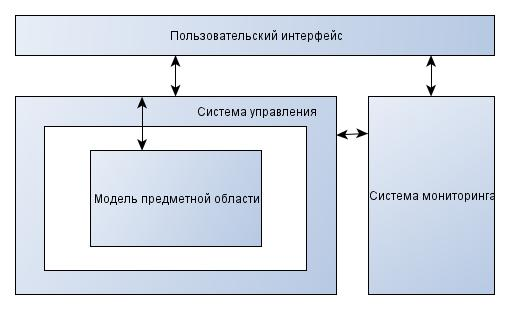
\includegraphics[width = 80mm]{Ch1Pic1}
        \caption{Представление разрабатываемой системы в виде совокупности взаимодействующих компонентов.} \label{Pic1}
    \end{figure}

\section{Выводы}

    Локальная сеть является динамически изменяющейся структурой. Эти изменения связаны с заменой оборудования, добавлением или удалением рабочих станций, смена используемого программного обеспечения и так далее. В некоторых случаях невозможно предусмотреть всех последствий, которые повлечет за собой то или иное изменение, и то может привести к появлению уязвимостей и нарушению безопасности системы. Для сведения к минимуму вероятности таких последствий на этапе разработки сети или в период, предшествующий изменениям, возможно провести испытания по безопасности на модели сети. 

    Моделирование сети позволяет провести исследование различных характеристик процесса функционирования сети, а так же проанализировать различные варианты изменений, которые необходимо внести в структуру сети и выбрать наиболее эффективный. Такой подход позволяет сократить расходы, к которым могут привести ошибочные решения, а так же время, за которое система сможет функционировать в нормальном режиме. 

    Для проведения моделирования сети могут быть использованы различные методы. Наиболее подходящим является метод имитационного моделирования, так как он позволяет изучить поведение системы с различными входными параметрами и проследить динамику изменения системы во времени. Кроме того, построение модели для имитационного моделирования является менее трудоемкой задачей, чем построение математической модели. Для этого могут быть использованы как специально разработанные языки имитационного моделирования, так и языки программирования общего назначения. 

    Для построения модели на языке имитационного моделирования требует от пользователя знания нюансов строения и функционирования различных узлов и протоколов сети, структуры и интенсивности генерации трафика пользователем, владения навыками построения моделей на каком-либо из языков имитационного моделирования. 

    Наиболее эффективным будет использование узкоспециализированной системы моделирования, которая предоставлет возможность пользователь задавать характеристики системы и ее отдельных узлов, при этом модели отдельных компонент предметной области будут включены в состав системы, что позволит в кратчайшие сроки строить модели различной степени сложности. 

    Таким образом, целью дипломного проекта является разработка системы моделирования сетевых атак. Эта система позволит инженеру по безопасности проводить испытания в различных условиях, таких как - нормальный режим и режимы для различных атак. Для достижения этой цели необходимо решить ряд задач:

\begin{itemize}
    \item исследование предметной области, выделение объектов для дальнейшего построения моделей;
    \item разработка моделей объектов и принципа их взаимодействия;
    \item реализация модели объектов с использованием языка программирования общего назначения;
    \item реализация вспомогательных систем, обеспечивающих возможности объединения моделей устройств в модель локальной сети, проведение испытаний, анализ результатов; 
\end{itemize}   
